\chapter{Specific Models}\label{chap:specific}

In the following part, we are going to propose several different ways
on how the edge weights are generated. And see how the two algorithms
proposed before can manage these situations.

\section{Ranking Model}

Consider the following model:
all the edge weights are independently sampled from the same distribution $D$ which is unknown to us.
The concept ``competitive ratio $\alpha$'' in this particular model
means that for any instance $G = (U, V, w)$ and distribution $D$,
by taking the expectation over all the possible weights and
all the permutations, we have $\frac{E[ALG]}{E[OPT]} \ge \alpha$.

Then there comes our first result.

\begin{theorem}\label{rothm}
    Simultaneous stopping rule achieves a constant competitive ratio.
\end{theorem}

As stated before, the problem for simultaneous stopping rule is, firms
have strong willings to compete with each other on those elite applicants
and less focus on those applicants who are not so outstanding but have
a safe position. So it's hard to grantee that each of them could
successfully hire a secretary. Here we will show that in the ranking model,
the chances of such collisions is rare.

In the following part, first we are going to state with high probability
that each firm $u$ would send an offer to its favorite applicant
-- the applicant with the highest score.
Then bound the probability that other firms would compete over its own
favorite applicant. Thus the probability for each firm to get its
best applicant is relatively high (at least a constant), which implies
the result.

Before the proof of this theorem, first we have to introduce some notations:
\begin{notation}\label{events}
    \ \\
\begin{itemize}
    \item Event $B(u_i, v_j)$ means that applicant $v_j$
        has the highest score with respect to firm $u_i$.
    \item Event $P(u_i, v_j)$ means that firm $u_i$ sends
        an offer to $v_j$.
    \item Event $A(u_i, v_j)$ means that firm $u_i$ sends
        an offer to $v_j$ and $v_j$ accepts it.
\end{itemize}

\end{notation}
\begin{proof}[Proof of Theorem~\ref{rothm}]
    WLOG let's assume that the incoming order of the applicants is
    $\{v_1, v_2, \dots, v_n\}$.

    Fix a particular firm $u \in U$,
    first bound the probability that it will get the best applicant
    with the highest score.
    \begin{align*}
        \Pr(u\text{ gets the best}) = &\sum_{i=1}^{n} \Pr(B(u, v_i)) \times \Pr(A(u, v_i)|B(u, v_i)) \\
                                = &\sum_{i=r}^{n} \frac{1}{n} \times \Pr(P(u, v_i)|B(u, v_i)) \\
                        & \times \Pr(A(u, v_i)|B(u, v_i),P(u, v_i))
    \end{align*}

    Given $v_i$ is the best applicant for $u$,
    once we ensure that the previous $(i-r)$ applicants are
    no better than the threshold, $u$ will be free when $v_i$ comes in
    and hence $u$ will send $v_i$ an offer.
    That is, we need to ensure that in the first $(i-1)$ applicants,
    the best of them is among the first $(r-1)$ ones.
    Given that all the applicants arrive in a random order,
    this probability would be simply $\frac{r-1}{i-1}$.
    Therefore

    $$\Pr(P(u, v_i) | B(u, v_i)) \ge \frac{r-1}{i-1}$$

    %$$\Pr(u\text{ gets the best}) \ge \sum_{i=r}^{n} \frac{1}{n} \times \frac{r-1}{i-1} \times \Pr(A(u, v_i)|B(u, v_i),P(u, v_i))$$


    As for the second part,
    if $v_i$ receives only one offer which is from $u$,
    $v_i$ can only choose $u$.
    And the condition holds when the score of $v_i$
    for each $u' \neq u$ does not exceed the threshold set by $u'$.
    In other words, for each $u' \neq u$, over the first $r-1$ applicants together with $v_i$,
    the best applicant for $u'$ is not $v_i$.
    These $m-1$ events (each with probability $\frac{r-1}{r}$) are independent from each other,
    and are all independent from $B(u, v_i)$ and $P(u, v_i)$.
    Thus
    $$\Pr(A(u, v_i)|B(u, v_i), P(u, v_i)) \ge \left(\frac{r-1}{r}\right)^{m-1}$$

    To sum up:
    $$\Pr(u\text{ gets the best}) \ge \sum_{i=r}^{n} \frac{1}{n} \times \frac{r-1}{i-1} \times \left(\frac{r-1}{r}\right)^{m-1}$$

    Let $p = \frac{r}{n}$ be a constant, and assume that $m \le \alpha n$ where $\alpha \in (0,1]$ is a parameter.

    Then $\left(\frac{r-1}{r}\right)^{m-1} \ge \left(1-\frac{1}{r}\right)^{\alpha n} = \left(\left(1-\frac{1}{r}\right)^{r}\right)^{\frac{\alpha}{p}}$ and

    $$\Pr(u \text{ gets the best}) \ge \left(\left(1 - \frac{1}{r}\right)^r\right)^{\frac{\alpha}{p}} \sum_{i=r}^{n} \frac{1}{n}\frac{r-1}{i-1}$$

    Now let $n$ goes to infinity and it is asymptotically the integral:

    $$f(p) = e^{-\frac{\alpha}{p}} \int_{p}^{1} \frac{p}{x} dx = -p \ln(p) e^{-\frac{\alpha}{p}}$$
    which is a constant depending on the choice of $p$.
    Thus, for each firm $u$, it
    has at least a constant probability $f(p)$ to get its best applicant, then we have
    \begin{align*}
        E[\text{score of the applicant }u\text{ gets in }ALG]
        & \ge f(p) \times E[\text{score of the best applicant for }u] \\
        & \ge f(p) \times E[\text{score of the applicant }u\text{ gets in }OPT]
    \end{align*}

    Therefore, it is clear to see that
    \[ \frac{E[ALG]}{E[OPT]} \ge f(p), \]
    and we did prove that the simultaneous stopping rule
    achieves a constant competitive ratio.
\end{proof}

Note that, in the analysis above, it is not necessary that all the weights
of edges are independently and identically distributed.
All we need is that firms' preference lists -- the order of applicants
according to the firm's score -- are sampled independently from each other.
That is, the rank of an applicant $v$ for a firm $u_i$ has nothing to do
with the rank of $v$ for another firm $u_j$.
So we named this model the \emph{ranking model}.

To generalize the ranking model above, we could weaken the restriction by
adding correlations between the weights of edges incident to
the same applicant, and introduce some new model.

\section{Gaussian Model}

In our daily lives, the score that firm $u$ grades $v$ is often dependent
on (i) the needs of $u$ and (ii) the inherent quality of $v$.
While the first one is usually uncertain and
hard to quantify. So in the following part,
we are going to discuss how the second term would affect firms' strategy.

Assume that each applicant has a quality $q_i$, and the weights of edges
incident to a certain applicant $v_i$ are generated independently from
a distribution $D_i$ with mean $q_i$.
As we can see, if all qualities are equal and all the distributions
are the same, then it is equivalent to the ranking model
discussed in the previous section.
Here we assume that $D_i$ is a gaussian distribution $N(q_i, \sigma^2)$
where $q_i$ is the inherent quality of applicant $v_i$ and the
standard deviation $\sigma$ is a fixed constant.

\subsection{Simultaneous stopping rule vs. Gaussian Model}\label{gaussian1}

As before, we formally define ``competitive ratio $\alpha$'' in this model --- for any given $G, \{q_i\}_{i=1}^n,$ and $\{D_i\}_{i=1}^n$, by taking the expectation over all the possible weights and all the permutations, we have $\frac{E[ALG]}{E[OPT]} \ge \alpha$.

First we have to define some parameters:
denote that $\delta_{max} = \max_{i \neq j} \abs{q_i - q_j}$ and
$\varphi = \frac{\delta_{max}}{\sigma}$. The following theorem holds.

\begin{theorem}\label{normalthm}
    Simultaneous stopping rule acheives a constant competetive ratio
    when $\varphi \le O(\frac{1}{n^2})$.
\end{theorem}

WLOG we assume that applicants arrive in the order of $\{v_1, v_2, \dots, v_n\}$,
and that for given qualities $\{q_i^\prime\}_{i=1}^n$, $\{q_i\}_{i=1}^n$ is a random permutation of $\{q_i^\prime\}_{i=1}^n$.
This is equivalent with the model where applicants arrive in a random order.

Together with the events which is defined in notation~\ref{events},
for $i \ge r$, let $D(u, v_i)$ be the event that $w(u, v_i)$
does not exceed the threshold set by $u$.

The proof of this theorem shares the same idea with the
one for Theorem~\ref{rothm}. We are going to argue that each firm has a large probability
to send its best applicant an offer, and with large probability no other
firm would propose to this special applicant.
The first two propositions below are established to ease the calculation,
and then follows the key lemma which directly implies the main theorem.

First of all we will introduce the error function we use in the analysis:
\begin{definition}
The error function
\[\mathrm{erf}(x) = \frac{2}{\sqrt{\pi}} \int_{0}^{x} {e^{-t^2}} \mathrm{d} t.\]
\end{definition}

\begin{figure} \centering
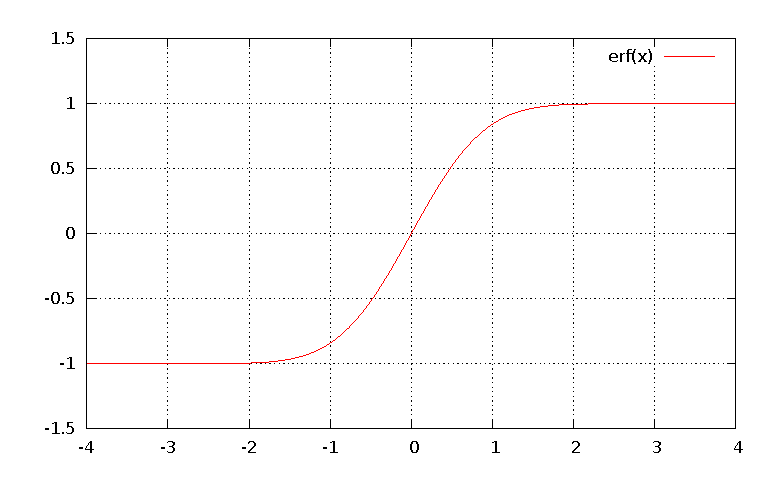
\includegraphics[width=0.8\textwidth]{figures/erf.eps}
\caption{Plot of error function}
\label{fig:errorfunction}
\end{figure}

This is a monotonically increasing function over $\mathbb{R}$ with value range $(-1, 1)$
as shown in figure~\ref{fig:errorfunction}.
It has some interesting properties. For example, it is related to the cumulative distribution 
$\Phi$ for gaussian distribution with mean $\delta$ and standard deviation $\sigma$:

\[\Phi(x) = \frac{1}{2} + \frac{1}{2}\erf \left( \frac{x - \delta}{\sqrt{2} \sigma} \right) \]

And the derivative of error function is

\[\frac{\mathrm{d}}{\mathrm{d}x}\erf(x) = \frac{2}{\sqrt{\pi}} e^{-x^2}\]

Then it is time to begin our proof.

\begin{proposition} \label{proposition1}
    For each $u \in U$ and $i \ge r$,
    \begin{align*}
    \Pr(D(u, v_i) | \{q_i\}_{i=1}^n) &\ge \Pr(D(u, v_i) | \forall 1 \le j \le r-1, q_j = q_i - \delta_{max}).
    \end{align*}
\end{proposition}

\begin{proof}
    For convience, let $x_i = w(u, v_i)$ be sampled from $N(q_i, \sigma^2)$.
    WLOG assume that $q_i = 0$.

    $D(u, v_i)$ means that there exists some $x_j$ such that $1 \le j \le r-1$ and $x_i < x_j$.

    \begin{align*}
        \Pr(D(u, v_i) | \{q_i\}_{i=1}^n) &= 1 - \int_{-\infty}^{\infty} \frac{1}{\sqrt{2 \pi}\sigma} e^{-\frac{x_i^2}{2\sigma^2}}
    \prod_{j=1}^{r-1} \left(\int_{-\infty}^{x_i} \frac{1}{\sqrt{2\pi}\sigma} e^{-\frac{(x_j - q_j)^2}{2\sigma^2}}\mathrm{d} x_j \right) \mathrm{d} x_i \\
    &= 1 - \int_{-\infty}^{\infty} \frac{1}{\sqrt{2 \pi}\sigma} e^{-\frac{x_i^2}{2\sigma^2}}
    \prod_{j=1}^{r-1}\left(\frac{1}{2} + \frac{1}{2}\mathrm{erf}\left(\frac{x_i - q_j}{\sqrt{2}\sigma}\right)\right) \mathrm{d} x_i,
    \end{align*}

    Now take derivative with respect to $q_j$:
    \begin{align*}
        & \frac{\partial\Pr(D(u, v_i) | \{q_i\}_{i=1}^n)}{\partial q_j} \\
        = &\int_{-\infty}^{\infty} \frac{1}{\sqrt{2 \pi}\sigma} e^{-\frac{x_i^2}{2\sigma^2}}
        \frac{1}{\sqrt{2 \pi} \sigma} e^{-\frac{(x_i-q_j)^2}{2\sigma^2}}
        \prod_{k<r,k\neq j}\left(\frac{1}{2} + \frac{1}{2}\mathrm{erf}\left(\frac{x_i - q_k}{\sqrt{2}\sigma}\right)\right) \mathrm{d} x_i
        \ge 0,
    \end{align*}
    which implies the result.
\end{proof}

\begin{proposition} \label{proposition2}
    For each $u \in U$ and $i \ge r$,
    $$ \Pr(D(u, v_i) | \forall 1 \le j \le r-1, q_j = q_i - \delta_{max}) \ge 1 - \frac{1}{r} - \frac{r - 1}{\sqrt{2\pi}}\varphi. $$
\end{proposition}

\begin{proof}
    First we have

    \begin{align*}
        &\Pr(D(u, v_i) | \forall 1 \le j \le r-1, q_j = q_i - \delta_{max}) \\
        = &1 - \int_{-\infty}^{\infty} \frac{1}{\sqrt{2 \pi}\sigma} e^{-\frac{x_i^2}{2\sigma^2}}
        \left(\frac{1}{2} + \frac{1}{2}\mathrm{erf}\left(\frac{x_i + \delta_{max}}{\sqrt{2}\sigma}\right)\right)^{r-1} \mathrm{d} x_i.
    \end{align*}
    Knowing that
    \begin{align*}
        & \frac{\mathrm{d} (\frac{1}{2} + \frac{1}{2} \mathrm{erf}(\frac{x}{\sqrt{2}\sigma}))^{r-1}}{\mathrm{d}x}\\
        = &\frac{r - 1}{\sqrt{2\pi}\sigma} e^{-\frac{x^2}{2\sigma^2}} \left(\frac{1}{2} + \frac{1}{2}\mathrm{erf}\left(\frac{x}{\sqrt{2}\sigma}\right)\right)^{r-2} \\
        \le &\frac{r-1}{\sqrt{2\pi}\sigma},
    \end{align*}
    by Mean Value Theorem, we have
    \begin{align*}
        \left(\frac{1}{2} + \frac{1}{2}\mathrm{erf}\left(\frac{x_i + \delta_{max}}{\sqrt{2}\sigma}\right)\right)^{r-1}
        &\le \left(\frac{1}{2} + \frac{1}{2}\mathrm{erf}\left(\frac{x_i}{\sqrt{2}\sigma}\right)\right)^{r-1}
        + \frac{r-1}{\sqrt{2\pi}\sigma} \times \delta_{max}.
    \end{align*}
    Therefore
    \begin{align*}
        & \int_{-\infty}^{\infty} \frac{1}{\sqrt{2 \pi}\sigma} e^{-\frac{x_i^2}{2\sigma^2}}
        \left(\frac{1}{2} + \frac{1}{2}\mathrm{erf}\left(\frac{x_i + \delta_{max}}{\sqrt{2}\sigma}\right)\right)^{r-1} \mathrm{d} x_i \\
        \le &\int_{-\infty}^{\infty} \frac{1}{\sqrt{2 \pi}\sigma} e^{-\frac{x_i^2}{2\sigma^2}}
        \left(\frac{1}{2} + \frac{1}{2}\mathrm{erf}\left(\frac{x_i}{\sqrt{2}\sigma}\right)\right)^{r-1} \mathrm{d} x_i \\
        & + \int_{-\infty}^{\infty} \frac{1}{\sqrt{2 \pi}\sigma} e^{-\frac{x_i^2}{2\sigma^2}}
        \frac{(r-1)\delta_{max}}{\sqrt{2\pi}\sigma}\mathrm{d} x_i.
    \end{align*}

    Note that the first term is exactly the probability that $x_i$ is the highest value among $\{x_k\}_{j=1}^{r-1} \cup \{x_i\}$, which equals $\frac{1}{r}$, and the second term
    \[\int_{-\infty}^{\infty} \frac{1}{\sqrt{2 \pi}\sigma} e^{-\frac{x_i^2}{2\sigma^2}}
        \frac{(r-1)\delta_{max}}{\sqrt{2\pi}\sigma}\mathrm{d} x_i
    = \frac{(r-1)\delta_{max}}{\sqrt{2\pi}\sigma}
    \int_{-\infty}^{\infty} \frac{1}{\sqrt{2 \pi}\sigma} e^{-\frac{x_i^2}{2\sigma^2}} \mathrm{d} x_i
    = \frac{(r-1)\delta_{max}}{\sqrt{2\pi}\sigma},\]
    thus
    \begin{align*}
    & \int_{-\infty}^{\infty} \frac{1}{\sqrt{2 \pi}\sigma} e^{-\frac{x_i^2}{2\sigma^2}}
        \left(\frac{1}{2} + \frac{1}{2}\mathrm{erf}\left(\frac{x_i + \delta_{max}}{\sqrt{2}\sigma}\right)\right)^{r-1} \mathrm{d} x_i \\
    = &\frac{1}{r} + \frac{r-1}{\sqrt{2\pi}} \frac{\delta_{max}}{\sigma} \\
    = &\frac{1}{r} + \frac{r - 1}{\sqrt{2\pi}} \varphi.
    \end{align*}
    
    Which implies the result.

\end{proof}

\begin{lemma} \label{cplem}
If every firm adopts simultaneous stopping rule, each of them can get
its best applicant with constant probability.
\end{lemma}

\begin{proof}
This is almost the same as Theorem~\ref{rothm}.
Fix a particular firm $u \in U$, we estimate the probability that $u$ gets
its best applicant.
\begin{align*}
    \Pr(u\text{ gets its best}|\{q_i\}_{i=1}^n) \ge \sum_{i=r}^{n} \frac{1}{n} \times \frac{r-1}{i-1}
                 \times \Pr(A(u, v_i) | B(u, v_i), P(u, v_i), \{q_i\}_{i=1}^n)
\end{align*}

Again if no other firm would send an offer to $v_i$, $A(u, v_i)$ must be true if $P(u, v_i)$ holds.
%Since the weights are generated independently, all events $\{P(u', v_i)| u' \in U\}$ are independent
%and $\{P(u', v_i) | u' \in U'\}$ are independent from $B(u, v_i)$ as long as $u \not\in U'$.
For any $u' \neq u$, $P(u', v_i)$ only depends on the value of $\{q_i\}_{i=1}^n$.
Thus, given $\{q_i\}_{i=1}^n$, all the events $\{P(u', v_i) | u' \neq u\}$ are independent from each other,
and are all independent from $B(u, v_i)$ and $P(u, v_i)$.
Therefore

\begin{align*}
    & \Pr(A(u, v_i) | B(u, v_i), P(u, v_i), \{q_i\}_{i=1}^n) \\
    \ge & \Pr(\bigcap_{u' \neq u}\overline{P(u', v_i)} | B(u, v_i), P(u, v_i), \{q_i\}_{i=1}^n) \\
    = & \prod_{u' \neq u} \Pr(\overline{P(u', v_i)} | \{q_i\}_{i=1}^n) \\
    \ge & \prod_{u' \neq u} \Pr(D(u', v_i) | \{q_i\}_{i=1}^n)
\end{align*}

Let $p = \frac{r}{n}$ be a constant, $\varphi \le \frac{c}{r(r-1)}$ for
some constant $c$ since $\varphi \le O(\frac{1}{n^2})$.
Then by proposition~\ref{proposition1} and~\ref{proposition2}
we have
\begin{align*}
\Pr(A(u, v_i) | B(u, v_i), P(u, v_i), \{q_i\}_{i=1}^n)
&\ge (1 - \frac{1}{r} - \frac{r - 1}{\sqrt{2\pi}}\varphi)^{m-1} \\
& \ge (1 - (1+\frac{c}{\sqrt{2\pi}})\frac{1}{r})^{m-1}
\end{align*}

Denote that $c' = 1 + \frac{c}{\sqrt{2\pi}}$.
Assume that $m \le \alpha n$ where $\alpha \in (0, 1]$ is a parameter.
To sum up, we have

\begin{align*}
    \Pr(u\text{ gets its best} | \{q_i\}_{i=1}^n)
    &\ge \sum_{i=r}^{n} \frac{1}{n} \times \frac{r-1}{i-1} \times (1 - \frac{c'}{r})^{m-1} \\
    &\ge ((1 - \frac{c'}{r})^{r})^{\frac{\alpha}{p}} \sum_{i=r}^{n} \frac{1}{n} \times \frac{r-1}{i-1}
\end{align*}

When $n$ goes to infinity, the summation above can be approximated by integral:
$$f(p) = e^{-\frac{c' \alpha}{p}}\int_{p}^{1} \frac{p}{x} \mathrm{d}x = -p\ln(p)e^{-\frac{c' \alpha}{p}}.$$
which is a constant.

Go back to the very beginning, where we are given a quality sequence $\{q_i^\prime\}_{i=1}^n$,
and $\{q_i\}_{i=1}^n$ is a random permutation of it. Thus we have when $n$ goes to infinity,
\begin{align*}
    & \Pr(u\text{ gets its best} | \{q_i^\prime\}_{i=1}^n) \\
    = &\sum \Pr (\{q_i\}_{i=1}^n | \{q_i^\prime\}_{i=1}^n) \times \Pr(u\text{ gets its best} | \{q_i\}_{i=1}^n) \\
    \ge & \sum \Pr (\{q_i\}_{i=1}^n | \{q_i^\prime\}_{i=1}^n) \times f(p) \\
    = & f(p)
\end{align*}

Therefore we have shown that, for each firm $u$, it has at least a constant probability to get its best applicant.
\end{proof}

With Lemma~\ref{cplem} we could know that simultaneous stopping rule is almost an optimal
strategy for each of the firms. 
It grantees that each firm could have a very good response with constant probability.
Now using the same analysis in Theorem~\ref{rothm},
it's sufficient to complete the proof of our main theorem.

%\begin{proof}[Proof of Theorem~\ref{normalthm}]
%\end{proof}


%In reality, it often comes that, all applicants' qualities fit in a
%constant range. Now if we let $\delta_{max}$ be a constant we have
%
%\begin{theorem}
%    Simultaneous stopping rule achieves a constant competitive ratio if
%    $\sigma \le O(\frac{1}{n})$ if all qualities fit in a constant range.
%\end{theorem}
%
%Here we just describe a sketch of the proof.
%
%First, weights of all except a constant number of edges lies in a constant
%range. This is because, for one particular edge, its weight $w_{i,j}$ is
%generated from $N(q_i, \sigma^2)$. By Chebyshev's Inequality, for any constant
%$c$, $\Pr(\abs{w_{i, j} - q_i} \ge c \times q_i) \le \frac{\sigma^2}{c^2 q_i^2}
%\le O(\frac{1}{n^2})$. So the expected number of edges whose weights
%fall out of a constant range is at most a constant.
%
%For those edges whose weights lie in a constant range, it doesn't matter
%which ones to be chosen. For others, there are only a constant number of
%edges which have threat for them. Which indicate a constant competitive
%ratio.

\subsection{Simultaneous stopping rule with $m$ slot vs. Gaussian Model}\label{gaussian2}

In the previous sections, we have got a rough idea that simultaneous stopping rule works well when the preference lists of all firms are ``different enough'' from each other.
Here preference list of a firm $u$ stands for the order of applicants 
according to the scores $u$ graded them.
Recall that in Example~\ref{example1}, this algorithm can get no better than $\Theta(\frac{\log n}{n})-$competitive ratio when the firms' view on the applicants are nearly identical to each other.
In this situation, we are going to claim that simultaneous stopping rule with $m$ slots can solve the problem.

With the same model define before, and correspondingly, we
define some parameters that $\delta_{min} = \min_{i \neq j} \abs{q_i - q_j}$, and
$\psi = \frac{\delta_{min}}{\sigma}$.
We claim that

%In the following discussion we assume that $q_1 \ge q_2 \ge \dots \ge q_n$.

\begin{theorem} \label{northm2}
    Simultaneous stopping rule with $m$ slots achieves a constant competitive
    ratio when $\psi \ge \omega(n)$ with large probability.
\end{theorem}

Here by saying ``achieves a constant competitive ratio with large probability" we mean:
with probability approaching 1 over all possible weights,
$\frac{E[ALG]}{E[OPT]} \ge c$ for some constant $c > 0$ where
the expectation is taken over all possible coming order of applicants.
We will break the proof of this theorem into two parts.
The first we are going to state that most of the time, firms will have the same preference
list according to the scores the graded applicants. And the second, in this situation, 
the best $m$ applicants would have large possibility of getting an offer.

\begin{lemma} \label{orderlem}
    When $\psi \ge \omega(n)$, for a given sequence $\{q_i\}_{i=1}^{n}$, with probability approaching 1 that
    each firm will have the same preference list of applicant as $\{q_i\}_{i=1}^{n}$

\end{lemma}

\begin{proof}
    For a particular firm $u$, %its edge weights $x_i$ are
    %sampled independently from $N(q_i, \sigma^2)$.
    denote $w(u, v_i)$ by $x_i$. Note that $x_i$ is sampled from $N(q_i, {\sigma}^2)$.
    What we are going to calculate is the probability that
    for any pair of $x_i$ and $x_j$ where $i \neq j$, $x_i < x_j$ iff $q_i < q_j$.

    WLOG, we assume $q_1 > q_2 > ... > q_n$. And we are going to give a lowerbound
    for $\Pr(x_1 > x_2 > \dots > x_n)$.
    \begin{align*}
        \Pr(x_1 > x_2 > \dots > x_n)
        & = \Pr(\bigcap_{i=2}^{n} (x_{i-1} > x_i)) \\
        & = 1 - \Pr(\bigcup_{i=2}^{n} (x_{i-1} > x_i)) \\
        & \ge 1 - \sum_{i=2}^{n} \Pr(x_{i - 1} \le x_i)
    \end{align*}

    Given that $q_i - q_{i-1} \ge \delta_{min}$,
    %$\Pr(x_{i-1} < x_i)$ is no more than $\Pr(b - a > \delta_{min})$
    %where $a$ and $b$ are sampled independently from $N(0, \sigma^2)$.
    we have
    \begin{align*}
    \Pr(x_{i-1} \le x_i) = & \Pr (x_i - x_{i-1} \geq 0) \\
    = & \Pr((x_i - q_i) - (x_{i-1} - q_{i-1}) \geq q_{i-1} - q_i) \\
    = & \Pr(a-b \geq q_{i-1} - q_i) \\
    \leq & \Pr(a-b \geq \delta_{min}),
    \end{align*}
    where $a$ and $b$ are sampled independently from $N(0, \sigma^2)$.

    Considering the random variable $a-b$, it's the same as the random variable $a+b$, i.e.,
    the sum of two identical normal distributions.
    Thus $a-b$ follows another normal distribution $N(0, 2\sigma^2)$.
    %The probability distribution for random variable $b-a$ is exactly
    %$N(0, 2\sigma^2)$ and symmetrical about 0.
    By Chebyshev's inequality:

    $$\Pr(x_i \le x_{i - 1}) \le \Pr(b - a \ge \delta_{min})
    = \frac{1}{2} \Pr(\abs{b-a} \ge \delta_{min}) \le \frac{\sigma^2}{\delta_{min}^2} = \frac{1}{\psi^2}$$

    To sum up we have

    $$\Pr(x_1 > x_2 > \dots > x_n) \ge 1 - \frac{n - 1}{\psi^2}$$

    Thus the probability that each firm has the same preference list as $\{q_i\}_{i=1}^{n}$
     is no less than $(1 - \frac{n-1}{\psi^2})^m$.
    Given that $m \le n$ and $\psi \ge \omega(n)$, this probability
    approaches 1 when $n$ goes to infinity.
\end{proof}

In the following part we assume that each firms has the same preference
list as $\{q_j\}_{i=1}^{n}$.
Then we are going to show that in this situation, the best $m$ applicants
could have a very good response -- being matched to their desired firms 
-- with high probability.

For convenience, we allow each firm to send offers even after it has been matched.
That is to say, it can still send virtual offers
(although virtual offers will be rejected all the time).
By our assumption, if an applicant receives an offer from a firm, 
every other firm would also send her an offer which might be virtual
according to the protocol. Since the preference list of all firms are 
identical. Note that, in the algorithm every firm sends out offers 
at most $m$ times, thus no more than $m$ applicants would have received 
offers. Which implies that once the applicant received offers, 
someone of them must be ``non-virtual" and the applicant could choose
the best offer among them.

Denote the set of all the applicants who receive offers by $S$. According to lemma~\ref{virtual} it is
proved
that for each applicant $v$ who is among the best $m$ applicants,
$\Pr(v \in S) \ge \frac{r}{n} \ln (\frac{n}{r})$ which
is a constant.

\begin{lemma} \label{finallem}
    If all firms have the same preference list as $\{q_i\}_{i=1}^{n}$,
    with constant probability,
    each of the best $m$ applicants (with highest qualities) will be matched to her best firm.
\end{lemma}

\begin{proof}
    Assume the incoming order of applicants is $\tau$, let
    $s_{\tau, i}$ be the $i$-th applicant who receives offers.
    %Fix a applicant $v_i$ where $i \le m$ is one of the best $m$ applicants.
    Fix an applicant $v$ who is one of the best $m$ applicants.

        Given that $s_{\tau, j} = v$, among $m$ offers $v$ has
    received, $j - 1$ of them are virtual and must be rejected.
    If the best offer for $v$ is among the left $m - j + 1$ ones, then $v$
    will get her best offer. Since all the weights of edges incident to $v$ are generated
    independently from the same distribution, this event happens with
    probability $\frac{m - j + 1}{m}$ and it is decreasing by the growth
    of $j$, therefore

    \begin{align*}
        \Pr(v_i\text{ gets her best} | v_i \in S) &= \sum_{j = 1}^{m}
        \Pr(s_{\tau, j} = v_i | v_i \in S) \times \frac{m - j + 1}{m}
        %&\ge \sum_{j=1}^{m} \frac{1}{m} \times \frac{m - j + 1}{m} \ge \frac{1}{2}
    \end{align*}

    We know that $\sum_{j = 1}^{m} \Pr(s_{\tau, j} = v_i | v_i \in S) = 1$.
    If we can show that $\Pr(s_{\tau, j} = v_i | v_i \in S)$ is also 
    decreasing by the growth of $j$, 
    by Chebyshev's sum inequality:

    $$\Pr(v_i\text{ gets her best} | v_i \in S) \ge \frac{1}{m} \sum_{j=1}^{m} \frac{m - j + 1}{m} \ge \frac{1}{2} $$

    Combine this with $\Pr(v \in S) \ge \frac{r}{n} \ln(\frac{n}{r})$ in lemma~\ref{virtual},
    and it's done.

    Now let's proof that $\Pr(s_{\tau, j} = v_i | v_i \in S)$ will decrease
    when $j$ becomes greater.
    For every $\tau$ where $s_{\tau, j} = v$ and $j > 1$, by swapping the
    position between $s_{\tau, j - 1}$ and $v$ we can obtain a new order $\tau'$.
    In this new incoming order, $v$ becomes the $(j-1)$-th to receive offers,
    i.e.,  by algorithm $s_{\tau', j - 1} = v$.
    Clearly, for two different coming order $\tau_1$ and $\tau_2$
    with $s_{\tau_1, j} = s_{\tau_2, j} = v$, the corresponding new orders
    $\tau_1'$ and $\tau_2'$ are also different.
    Thus $|\{\tau | s_{\tau, j-1} = v\}| \geq |\{\tau | s_{\tau, j} = v\}|$.
    Therefore
    $\Pr_{\tau}(s_{\tau, j - 1} = v | v \in S)
    \ge \Pr_{\tau}(s_{\tau, j} = v | v \in S)$ for all $j > 1$.
\end{proof}

\begin{proof}[Proof of Theorem~\ref{northm2}]
    With Lemma~\ref{orderlem}, what we need to show is that
    given all firms have the same preference list as $\{q_i\}_{i=1}^{n}$,
    $\frac{E[ALG]}{E[OPT]} \ge c$ for some constant $c > 0$.

    Denote the set of the best $m$ applicant by $T$.

    In this situation, $E[OPT] \le \sum_{v_i \in T} \max_{u \in U} w(u, v_i)$.

    According to Lemma~\ref{finallem}, the algorithm grantees that for every $v_i \in T$,
    she will be matched to her best firm with constant probability.
    Which means $E[ALG] \ge \sum_{v_i \in T} c \times \max_{u \in U} w(u, v_i)$ for some constant $c > 0$.

    Which implies the result.
\end{proof}

\begin{corollary}
    Each firm has a probability of $\Omega(\frac{1}{m})$ to obtain
    the best applicant.
\end{corollary}

\begin{proof}
By Lemma~\ref{orderlem}, with probability approaching 1 that all firms consider the same applicant as the best.
Denote the best applicant by $v$. By the fact that $Pr(v \in S) \ge \frac{r}{n} \ln(\frac{n}{r})$ is a constant,
$v$ would be matched to some firm with constant probability.
Since there is no difference between the firms, each firm has a probability of $\frac{1}{m}$ to be chosen.
\end{proof}

Note that in this setting all firms are facing nearly the same situation.
Because every firm wants good applicants and here ``good" means
almost the same for them.
When competing with other firms, the result relies more on applicant's
choice instead of their own strategies.

\section{Future works}

In the section of Gaussian model, we discussed two ways on how the edge
weights are generated. 
In section~\ref{gaussian1} we showed that if the ``correlation" between
the scores of one applicant is weak enough -- i.e.\ the preference lists of
firms are highly distinguished -- simultaneous stopping rule
would do a good job. On the other hand, in section~\ref{gaussian2}, if
the distributions of one applicant's scores are highly correlated --
i.e.\ the preference lists of firms are quite similar -- by extending 
the size of threshold set simultaneous stopping rule with $m$
slots could achieve a good performance.

So intuitively we believe that there is a relation between how similar
the firms' preference lists are and how many thresholds each 
firm should set. For example, 1 for all preference lists are totally 
independent, $m$ for
they are the nearly the same to obtain a constant competitive ratio for both
social welfare and individuals.

It will be interesting to dig out a correlation parameter between the firms'
preference lists. And hopefully the following conjecture will hold.

\begin{conjecture}
    Under the framework of simultaneous stopping rule, there exists 
    a function $f$ and a parameter $\rho$ which depends only on 
    the distributions of the edge weights such that, 
    simultaneous stopping rule with $f(\rho)$ slots could achieve a
    constant competitive ratio.
\end{conjecture}

%Before making conjecture, we find out a parameter for two particular
%distributions.
